\section{Acquiring Data (Model Cell Tutorial)}

This section presents a tutorial similar to those described by Molecular Devices for their suite of electrophysiology products. This exercise uses a CLAMP-1U model cell with an Axon\tm Axoclamp\tm 2B amplifier operating in bridge mode. Connect the HS-2A-x0.1LU headstage to the ME1 PROBE connector and the HS-2A-x1LU head stage to the ME2 probe connector on the back panel of the amplifier.

\marginlabel{Connect equipment\\to DAQ card} Make the following connections between the amplifier and the DAQ card. 
\begin{enumerate}
\item Axoclamp 10Vm Output $\rightarrow$ DAQ Analog Input 0
\item Axoclamp Im Output $\rightarrow$ DAQ Analog Input 1
\item DAQ Analog Output 0 $\rightarrow$ Axoclamp EXT. ME1 COMMAND
\end{enumerate}

\marginlabel{Start RTXI} If you have not already calibrated your DAQ card, use \texttt{comedi\_calibrate} or \texttt{comedi\_soft\_calibrate} (if you have an NI M-series card):
\begin{example}
\$ sudo comedi\_calibrate --reset --dump --calibrate --results --verbose /dev/comedi0
\end{example}
If you installed RTXI using the Live CD, you may start RTXI from the Applications menu. However, it is a good idea to start RTXI from the terminal since some modules output error messages or warnings to the terminal: 
\begin{example}
\$ rtxi
\end{example}
\vspace{1cm}
\marginlabel{Configure DAQ Channels} \index{DAQ, configuration}While RTXI automatically detects the available channels on your DAQ card, they need to be configured inside RTXI. From the \textbf{System} menu on the RTXI menu bar, choose the \textbf{Control Panel}. The default device should be your DAQ card listed as \texttt{/dev/comedi0}. The analog channels on most multifunction DAQ cards have a range of -10 V to +10 V based on a ground reference and this is the default in RTXI. You should check the specifications for your DAQ card and choose the corresponding settings in RTXI. For Analog Input 0, the amplifier specifies that the signal has a gain of 10 applied (10Vm). Invert this and enter a scale of 0.1 V/V for this channel. Click the \textbf{``Active"} toggle button and click the \textbf{``Apply"} button. You will not acquire any actual data on a channel until it has been set to ``Active."
\begin{figure}[h]
\begin{center}
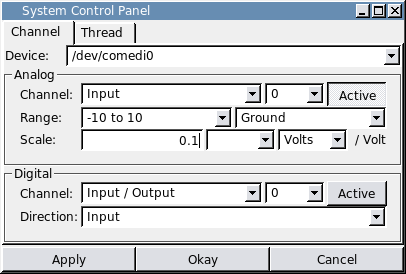
\includegraphics[width=4in]{axoclamptutorial0.png} 
\caption[Axoclamp Tutorial: Analog Input 0]{Configuring Axoclamp 10Vm output on Analog Input 0} 
\end{center}
\label{fig:axoclamptutorial0}
\end{figure}

\newpage For the membrane current assigned to Analog Input 1, the Axoclamp amplifier specifies that there is a gain of 10 $\div$ H mV/nA. Since the headstage gain on ME1 is H=0.1, the conversion is 100 mV/nA or 0.1 V/nA. Invert this to get a scale of 10 nA/V. You may set the ``Scale" dropdown box to either units of volts or amperes but this does not affect the computation. \attention Note that you must compute the total gain applied to a channel by any combination of hardware and software along the path of the signal. For example, if you are using the Axon\tm Multiclamp\tm Microelectrode Amplifier by Molecular Devices, you should take into account Multiclamp Commander software gain.

\begin{figure}[h]
\begin{center}
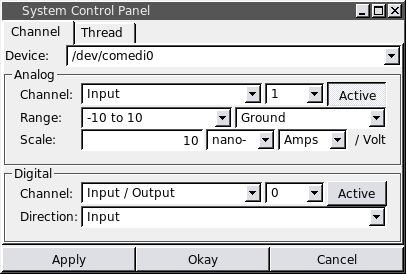
\includegraphics[width=4in]{axoclamptutorial1.png} 
\caption[Axoclamp Tutorial: Analog Input 1]{Configuring Axoclamp Im output on Analog Input 1} 
\end{center}
\label{fig:axoclamptutorial1}
\end{figure}
\vspace{1.5cm}

For the EXT. ME1 COMMAND assigned to Analog Output 0, the Axoclamp specified a gain of 10 x H nA/V, which comes to 1 nA/V. Invert this to get a scale of 1 gigaV/A.

\begin{figure}[h]
\begin{center}
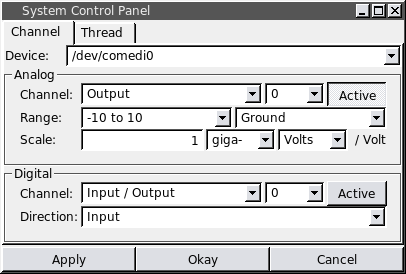
\includegraphics[width=4in]{axoclamptutorial2.png} 
\caption[Axoclamp Tutorial: Analog Output 0]{Configuring EXT. ME1 COMMAND on Analog Output 0}
\end{center}
\label{fig:axoclamptutorial2}
\end{figure}

\attention The Thread Tab of the System Control Panel allows you to set the real-time period or sampling rate \index{sampling rate} of the system. The default sampling rate is 1 kHz, which is sufficient for this exercise.

\vspace{1cm}
\marginlabel{Configure stimulus module} The Istep module generates  current step stimuli (square wave pulses). Install the Istep module according to the directions in Chapter \ref{module installation} and load it by selecting \textbf{Modules}$\rightarrow$\textbf{Load Modules} from the RTXI menu bar. Set the amplitude of the current pulse to 5 nA and set the width of the pulse to 40 ms using the Period and Duty Cycle options. The number of pulses is set using the Cycles option.

\begin{figure}[h]
\begin{center}
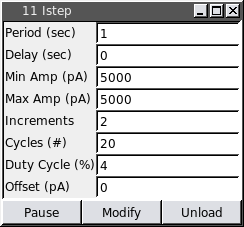
\includegraphics[width=2.2in]{istep.png} 
\caption[Istep]{The Istep module delivers current step pulses.} 
\end{center}
\label{fig:istep}
\end{figure}

\vspace{1cm}
\marginlabel{Configure Oscilloscope}Start the Oscilloscope by selecting \textbf{System}$\rightarrow$\textbf{Oscilloscope} from the RTXI menu bar. Right click anywhere in the Oscilloscope window to bring up the context menu and select the \textbf{Properties} menu. \seealso{Chapter \ref{Oscilloscope}\\Oscilloscope}The \textbf{Channel Tab} is used to select signals to plot and set an appropriate scale and line style. The architecture of RTXI is based on modular components that have input and output signals. \attention The DAQ card is abstracted as a DAQ device block such that a signal acquired on an input channel of the DAQ \emph{card} becomes an output signal of the DAQ \emph{device} within RTXI. To plot the voltage acquired on Analog Input 0, use the dropdown box to select \textbf{``Output"}. The rightmost dropdown box will automatically be populated with the analog input channels of the DAQ card. Click the \textbf{``Active"} toggle button to plot the signal. 

\begin{figure}[h]
\begin{center}
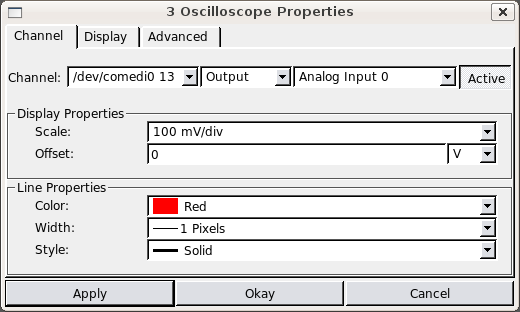
\includegraphics[width=4.5in]{oscilloscope1.png} 
\caption[Oscilloscope]{The Oscilloscope Channel Tab allows you to select signals to plot and choose different scales and line styles.} 
\end{center}
\end{figure}

When a signal is plotted, the Oscilloscope will generate a legend in the lower part of the window. In the \textbf{Display Properties} section, choose a scale and if needed, an offset. You may also choose a linestyle in the \textbf{Line Properties} section. You must click the \textbf{Apply} button for these changes to take effect. Each signal may have a different scale and different line style. Use the System Control Panel to plot Analog Input 0 and Analog Input 1 to monitor the voltage and the current applied to the model cell. You should also plot the ``Iout" output signal of the Istep module.

\vspace{1cm}
\marginlabel{Connect Signals\\Within RTXI}To generate signals from the Istep module, untoggle the \textbf{``Pause"} button. RTXI will begin executing the real-time code specified in this module. You should see pulses in the Istep signal in the Oscilloscope window. You can use the textboxes in the GUI to change the parameter values. The text will turn red but there will be no change in the module's output signal until you click the \textbf{``Modify"} button. Clicking this button initiates an event that will update the parameter in real-time and you should see the corresponding change immediately in the Oscilloscope. At this point, you  should not see any pulses in Analog Input 1 from your DAQ card, which is the current actually delivered by the amplifier. To apply this stimulus to the model cell, you need to make a connection between the Istep module and the DAQ card. From the RTXI menu bar, select \textbf{System}$\rightarrow$\textbf{Connector}. 

\begin{figure}[h]
\begin{center}
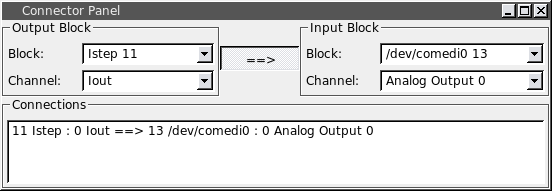
\includegraphics[width=4.5in]{connector1.png} 
\caption[Connector]{The Connector allows you to create connections between user modules or between modules and the DAQ card.} 
\end{center}
\end{figure}

The Connector module populates the \textbf{``Output Block"} with the available signals in your workspace and the \textbf{``Input Block"} with the available slots, or destinations. Select the Istep module in the ``Output Block" and the ``Iout" signal. Choose your DAQ card (\texttt{/dev/comedi0}) in the ``Input Block" and the Analog Output 0 channel. To make the connection, click the central ``==$>$" toggle button. Now, the Oscilloscope should show matching data for both Istep: Iout and Analog Input 1.

\vspace{1cm}
\marginlabel{Balance the Bridge\\ in the Bath}
Switch the CLAMP-1U model cell to the BATH position. Use the amplifier INPUT OFFSET knob to zero out the voltage based on the readings in the Oscilloscope. The Oscilloscope shows the actual sample values (with the channel gain applied) that will later be saved using the Data Recorder module. If your amplifier or other control software indicates a nonzero voltage when RTXI reports a zero voltage, \seealso{Chapter \ref{comedi calibration}\\COMEDI calibration}calibrating your DAQ card may eliminate this offset. Unpause the Istep module to begin delivering current pulses to the model cell. Adjust the BRIDGE knob until the voltage deflection is eliminated and then adjust the CAPACITANCE NEUTRALIZATION knob until the residual transients are minimized. Now switch the model cell to the CELL position. If you have correctly tuned these settings, you should see a response to each current pulse as in Figure \ref{balancedbridge}.

\begin{figure}[h!]
\begin{maxipage}
\begin{center}
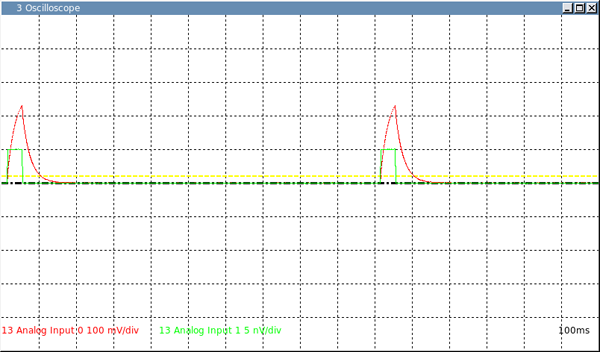
\includegraphics[width=5.2in]{axoclamptutorial3.png} 
\caption[Axoclamp Tutorial: Balanced Bridge]{Model cell response to current injection pulses with correctly balanced bridge and capacitance neutralization}
\label{fig:balancedbridge}
\end{center}
\end{maxipage}
\end{figure}

\begin{figure}[h!]
\begin{maxipage}
\begin{center}
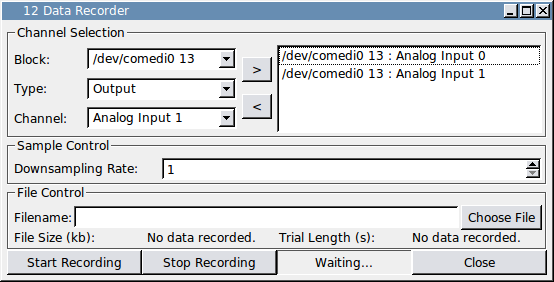
\includegraphics[width=5in]{axoclamptutorial4.png} 
\caption[Data Recorder]{The Data Recorder saves any synchronous signal in your workspace to an HDF5 file.} 
\end{center}
\end{maxipage}
\end{figure}

\marginlabel{Saving Data}To record data, select \textbf{System}$\rightarrow$\textbf{Data Recorder} from the RTXI menu bar. The \textbf{``Block"} menu is a list of your DAQ card(s) and any loaded user modules. Selecting a block device then populates the \textbf{``Type"} and \textbf{``Channel"} menus. Select the Analog Input 0 channel from your DAQ device and click the \textbf{``$>$"} button. To remove a channel from the list, highlight it in the listbox and click the \textbf{``$<$"} button. Before you can start recording, you must select a file by clicking the \textbf{``Choose File"} button. Click \textbf{``Start Recording"} to begin recording and \textbf{``Stop Recording"} to stop recording.

\vspace{1cm}
\marginlabel{Saving Your Workspace}
At this point, you have configured several channels on the DAQ card and the Oscilloscope, set custom parameters for a user module, and connected the module to the DAQ card to generate an external signal. RTXI allows you to save all these settings to a file by selecting \textbf{File}$\rightarrow$\textbf{Save Workspace} from the RTXI menu bar. To reload the file and reconstruct your entire working environment, select   \textbf{File}$\rightarrow$\textbf{Load Workspace}.